% This is samplepaper.tex, a sample chapter demonstrating the
% LLNCS macro package for Springer Computer Science proceedings;
% Version 2.20 of 2017/10/04
%

\documentclass[runningheads]{llncs}
%
\usepackage[utf8]{inputenc}
\usepackage[utf8]{vietnam}
\usepackage{graphicx}
\usepackage{epstopdf}
% Used for displaying a sample figure. If possible, figure files should
% be included in EPS format.
%
% If you use the hyperref package, please uncomment the following line
% to display URLs in blue roman font according to Springer's eBook style:
% \renewcommand\UrlFont{\color{blue}\rmfamily}

\begin{document}
%
\title{Xây dựng bộ dữ liệu Hỏi đáp cho Tiếng Việt về COVID-19\thanks{Hướng dẫn bởi TS. Nguyễn Gia Tuấn Anh và CN. Lưu Thanh Sơn}}
%
%\titlerunning{Abbreviated paper title}
% If the paper title is too long for the running head, you can set
% an abbreviated paper title here
%
\author{Thái Minh Triết\inst{1} \and
Chu Hà Thảo Ngân\inst{2} \and
Võ Tuấn Anh\inst{3} \and
Lưu Thanh Sơn\inst{5} \and
Nguyễn Lưu Tuấn Anh\inst{4} 
}
%
\authorrunning{Thái Minh Triết, Chu Hà Thảo Ngân , Võ Tuấn Anh}
% First names are abbreviated in the running head.
% If there are more than two authors, 'et al.' is used.
%
\institute{Trường Đại học Công nghệ thông tin, Đại học quốc gia Thành phố Hồ Chí Minh \and
Khoa Khoa học và Kỹ thuật Thông tin\\
\email{\{\inst{1}19522397,\inst{2}19521882,\inst{3}19521226\}@gm.uit.edu.vn\\
{\{\inst{4}sonlt,\inst{5}anhngt}\}@uit.edu.vn}}

%\institute{Trường Đại học Công nghệ Thông tin, Đại học Quốc gia Thành phố Hồ chí Minh
%\\ Khoa Khoa học và Kỹ thuật Thông tin
%\\ \email{\{19522397,19521882,19521226\}@gm.uit.edu.vn}}
%
\maketitle              % typeset the header of the contribution
%
\begin{abstract}
Tính đến ngày 21 - 06 - 2021, dịch COVID-19 đã xuất hiện tại 40 tỉnh thành của Việt Nam với hơn 10.000 ca nhiễm. Trước tình hình này, Trung tâm kiểm soát \& phòng ngừa dịch bệnh, Học viên Quân Y và các tổ chức y tế công cộng đã nhanh chóng biên soạn những bộ tài liệu hỏi đáp nhằm giải đáp thắc mắc của cộng đồng về COVID-19 và các vấn đề liên quan.
Với mong muốn giúp người dân Việt Nam có thể dễ dàng tiếp cận thông tin về COVID-19 và các chính sách phòng chống dịch, chúng tôi tiến hành thu nhập các câu hỏi đáp Tiếng Việt từ website của các tổ chức y tế, trung tâm y tế công cộng và Cổng thông tin điện tử Chính phủ. Sau đó tiền xử lý, đánh giá và đưa ra bộ dữ liệu sạch để giúp cho cộng đồng có thể tra cứu thông tin về COVID-19 và các chính sách của chính phủ trong bối cảnh dịch bệnh còn đang diễn biến phức tạp. Trong tương lai, bộ dữ liệu có thể được sử dụng cho việc xây dựng các mô hình Hỏi đáp tự động, qua đó giúp người dân có thể tiếp cận thông tin một cách nhanh chóng và thuận tiện hơn.


\keywords{COVID-19  \and Thu thập dữ liệu \and Q\&A Dataset\and Tidy Data.}
\end{abstract}
%
%
%
\section{Giới thiệu chung}

Sự bùng phát dịch bệnh COVID-19 được tuyên bố là tình trang y tế cộng đồng khẩn cấp, virus này đã lây lan nhiều quốc gia và nhiều vùng lãnh khổ, đây là tình trạng gây quan ngại quốc tế. Việc cộng đồng nắm được thông tin và diễn biến của COVID-19 đóng vai trò quan trọng, giúp cộng đồng hiểu rõ về dịch bệnh, giảm đi sự lo lắng cũng như có kiến thức cho cộng đồng hành động ngăn ngừa sự lan rộng của dịch bệnh.

Trước tình hình này, Tổ chức Y tế Thế giới WHO, Trung tâm kiểm soát \& phòng ngừa dịch bệnh CDC, Bộ Y tế, Học viện Quân Y và nhiều Cổng thông tin y tế điện tử đã nhanh chống biên soạn tài liệu hướng dẫn kỹ thuật và giáo dục cộng đồng cho hoạt động phòng chống COVID-19. Tuy trong bối cảnh nội dung số phát triển hiện nay, nhu cầu tìm kiếm, tra cứu và truy xuất thông tin chính xác, đầy đủ và kịp thời là hơn bao giờ hết, nhưng phần lớn người dân Việt Nam còn gặp nhiều khó khăn để có thể tiếp cận những nguồn tin chính thống tiếng Việt để giải đáp những thắc mắc của mình về đại dịch và các chính sách liên quan.
Với mong muốn cung cấp thông tin cho người dân một cách nhanh chóng, rõ ràng và chính xác, chúng tôi tiến hành xây dựng bộ dữ liệu Hỏi đáp cho Tiếng Việt về COVID-19 để phục vụ cho bài toán tra cứu cũng như bài toán Hỏi đáp tự động trong tương lai.

Thách thức của bài toán chúng tôi là xây dựng một bộ dữ liệu phải có tính nhất quán, chính xác và kịp thời các thông tin về vấn đề COVID-19 hiện nay. Từ kết quả đạt được, bộ dữ liệu chúng tôi đã xây dựng nhằm mục đích cung cấp thông tin về COVID-19 và chính sách liên quan đến cộng đồng một cách rõ ràng, mang tính hành động trong công tác ngăn ngừa, phát hiện sớm và kiểm soát COVID-19 trong cộng đồng.

Trong bài báo cáo này, chúng tôi tập trung xây dựng bộ dữ liệu từ những câu hỏi đáp thường gặp về COVID-19 trên ngôn ngữ tiếng Việt. Cấu trúc bài báo cáo được trình bày như sau: Ở mục 2, chúng tôi trình bày chi tiết phương pháp thu nhập và quá trình xây dựng bộ dữ liệu. Ở mục 3, chúng tôi tiếp cận bộ dữ liệu và thực hiện tiền xử lý dữ liệu. Kết quả chúng tôi thu được là bộ dữ liệu tidy data sẽ được trình bày ở mục 4. Và cuối cùng ở mục 5 là kết luận và hướng phát triển.

\section{Phương pháp thu nhập}

\section{Tiền xử lý dữ liệu}

\section{Bộ dữ liệu tidy data}

\section{Kết luận và hướng phát triển}
\subsection{A Subsection Sample}
Please note that the first paragraph of a section or subsection is
not indented. The first paragraph that follows a table, figure,
equation etc. does not need an indent, either.

Subsequent paragraphs, however, are indented.

\subsubsection{Sample Heading (Third Level)} Only two levels of
headings should be numbered. Lower level headings remain unnumbered;
they are formatted as run-in headings.

\paragraph{Sample Heading (Fourth Level)}
The contribution should contain no more than four levels of
headings. Table~\ref{tab1} gives a summary of all heading levels.

\begin{table}
\caption{Table captions should be placed above the
tables.}\label{tab1}
\begin{tabular}{|l|l|l|}
\hline
Heading level &  Example & Font size and style\\
\hline
Title (centered) &  {\Large\bfseries Lecture Notes} & 14 point, bold\\
1st-level heading &  {\large\bfseries 1 Introduction} & 12 point, bold\\
2nd-level heading & {\bfseries 2.1 Printing Area} & 10 point, bold\\
3rd-level heading & {\bfseries Run-in Heading in Bold.} Text follows & 10 point, bold\\
4th-level heading & {\itshape Lowest Level Heading.} Text follows & 10 point, italic\\
\hline
\end{tabular}
\end{table}


\noindent Displayed equations are centered and set on a separate
line.
\begin{equation}
x + y = z
\end{equation}
Please try to avoid rasterized images for line-art diagrams and
schemas. Whenever possible, use vector graphics instead (see
Fig.~\ref{fig1}).

\begin{figure}
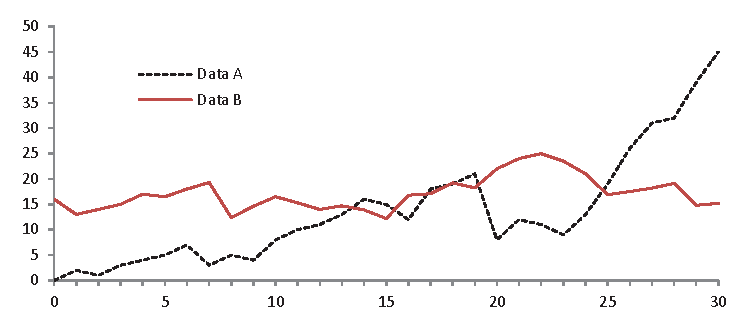
\includegraphics[width=\textwidth]{fig1.eps}
\caption{A figure caption is always placed below the illustration.
Please note that short captions are centered, while long ones are
justified by the macro package automatically.} \label{fig1}
\end{figure}

\begin{theorem}
This is a sample theorem. The run-in heading is set in bold, while
the following text appears in italics. Definitions, lemmas,
propositions, and corollaries are styled the same way.
\end{theorem}
%
% the environments 'definition', 'lemma', 'proposition', 'corollary',
% 'remark', and 'example' are defined in the LLNCS documentclass as well.
%
\begin{proof}
Proofs, examples, and remarks have the initial word in italics,
while the following text appears in normal font.
\end{proof}
For citations of references, we prefer the use of square brackets
and consecutive numbers. Citations using labels or the author/year
convention are also acceptable. The following bibliography provides
a sample reference list with entries for journal
articles~\cite{ref_article1}, an LNCS chapter~\cite{ref_lncs1}, a
book~\cite{ref_book1}, proceedings without editors~\cite{ref_proc1},
and a homepage~\cite{ref_url1}. Multiple citations are grouped
\cite{ref_article1,ref_lncs1,ref_book1},
\cite{ref_article1,ref_book1,ref_proc1,ref_url1}.
%
% ---- Bibliography ----
%
% BibTeX users should specify bibliography style 'splncs04'.
% References will then be sorted and formatted in the correct style.
%
% \bibliographystyle{splncs04}
% \bibliography{mybibliography}
%
\begin{thebibliography}{8}
\bibitem{ref_article1}
Author, F.: Article title. Journal \textbf{2}(5), 99--110 (2016)

\bibitem{ref_lncs1}
Author, F., Author, S.: Title of a proceedings paper. In: Editor,
F., Editor, S. (eds.) CONFERENCE 2016, LNCS, vol. 9999, pp. 1--13.
Springer, Heidelberg (2016). \doi{10.10007/1234567890}

\bibitem{ref_book1}
Author, F., Author, S., Author, T.: Book title. 2nd edn. Publisher,
Location (1999)

\bibitem{ref_proc1}
Author, A.-B.: Contribution title. In: 9th International Proceedings
on Proceedings, pp. 1--2. Publisher, Location (2010)

\bibitem{ref_url1}
LNCS Homepage, \url{http://www.springer.com/lncs}. Last accessed 4
Oct 2017
\end{thebibliography}
\end{document}
